\section{Problem 6}
State space to transfer function.

In general, state space representations are not unique as discussed in lecture. You are given the following systems.


    \begin{align}
        \begin{bmatrix}
            \dot{x} \\
            \ddot{x}
        \end{bmatrix} &=
        \begin{bmatrix}
            -5 & 0 \\
            0  & -1
        \end{bmatrix}
        \begin{bmatrix}
            x \\
            \dot{x}
        \end{bmatrix} + 
        \begin{bmatrix}
            3\\
            1
        \end{bmatrix}
        u \label{eq:16}
        \\
        y &=
        \begin{bmatrix}
            7 & 0
        \end{bmatrix}
        \begin{bmatrix}
            x \\
            \dot{x}
        \end{bmatrix} \label{eq:17}
    \end{align}



\begin{align}
    \begin{bmatrix}
        \dot{x} \\
        \ddot{x}
    \end{bmatrix} &=
    \begin{bmatrix}
        -5 & 0 \\
        0  & -1
    \end{bmatrix}
    \begin{bmatrix}
        x \\
        \dot{x}
    \end{bmatrix} + 
    \begin{bmatrix}
        3\\
        0
    \end{bmatrix}
    u\label{eq:18}
    \\
    y &=
    \begin{bmatrix}
        7 & 3
    \end{bmatrix}
    \begin{bmatrix}
        x \\
        \dot{x}
    \end{bmatrix}\label{eq:19}
\end{align}

\subsection{a)}
Analytically (by hand!) show that these systems will result in the same transfer
function $\frac{Y(s)}{U(s)}$.
\subsubsection{\textit{ Sol. }}

Start by doing Laplace transform on state equation in Eq.\ref{eq:16} and Eq.\ref{eq:17}:

\begin{align}
    \mathcal{L} \{\dot{\textbf{x}}\} &= sX(s) = AX(s) + BU(s) \label{eq:20}\\ 
    \mathcal{L} \{y\} &= Y(s) = CX(s) + DU(s) \label{eq:21}
\end{align}
From Eq.\ref{eq:20} we get:
\begin{equation}
    X(s) = (sI - A)^{-1}BU(s) \label{eq:22}
\end{equation}

Replace $X(s)$ in Eq.\ref{eq:21} with Eq.\ref{eq:22}
\begin{equation}
    Y(s) = (C(sI - A)^{-1}B + D)U(s) \label{eq:23}
\end{equation}
So we have: 
\begin{equation}
    \begin{aligned}
        \frac{Y(s)}{U(s)} &= C(sI - A)^{-1}B + D \\
        &= \begin{bmatrix} 7 & 0 \end{bmatrix}
        (\begin{bmatrix} s & 0 \\ 0 & s \end{bmatrix} -
        \begin{bmatrix} -5 & 0 \\ 0 & -1 \end{bmatrix})^{-1}
        \begin{bmatrix} 3\\1\end{bmatrix} + 0 \\ 
        &= \begin{bmatrix} 7 & 0 \end{bmatrix}\left(\frac{1}{(s+1)(s+5)}\begin{bmatrix}
            s+1 & 0 \\
            0   & s+5
        \end{bmatrix}\right)\begin{bmatrix} 3\\1\end{bmatrix}\\ 
        &= \begin{bmatrix} 7 & 0 \end{bmatrix}\begin{bmatrix} \frac{3}{(s+5)} \\ \frac{1}{(s+1)} \end{bmatrix}\\ 
        &=\frac{21}{s+5}
    \end{aligned}
\end{equation}

Now we do the same to Eq.\ref{eq:18} and Eq.\ref{eq:19}:
\begin{equation}
    \begin{aligned}
        \frac{Y(s)}{U(s)} &= C(sI - A)^{-1}B + D \\
        &= \begin{bmatrix} 7 & 3 \end{bmatrix}
        (\begin{bmatrix} s & 0 \\ 0 & s \end{bmatrix} -
        \begin{bmatrix} -5 & 0 \\ 0 & -1 \end{bmatrix})^{-1}
        \begin{bmatrix} 3\\0\end{bmatrix} + 0 \\ 
        &= \begin{bmatrix} 7 & 3 \end{bmatrix}\left(\frac{1}{(s+1)(s+5)}\begin{bmatrix}
            s+1 & 0 \\
            0   & s+5
        \end{bmatrix}\right)\begin{bmatrix} 3\\0\end{bmatrix}\\ 
        &= \begin{bmatrix} 7 & 3 \end{bmatrix}\begin{bmatrix} \frac{3}{(s+5)} \\ 0 \end{bmatrix}\\ 
        &=\frac{21}{s+5}
    \end{aligned}
\end{equation}

We get the same transfer function $\frac{Y(s)}{U(s)} = \frac{21}{s+5}$.

\subsection{b)}
Matlab code:
    \lstinputlisting{codes/Question6b.m}
Result:
\begin{figure}[htp]
    \centering
    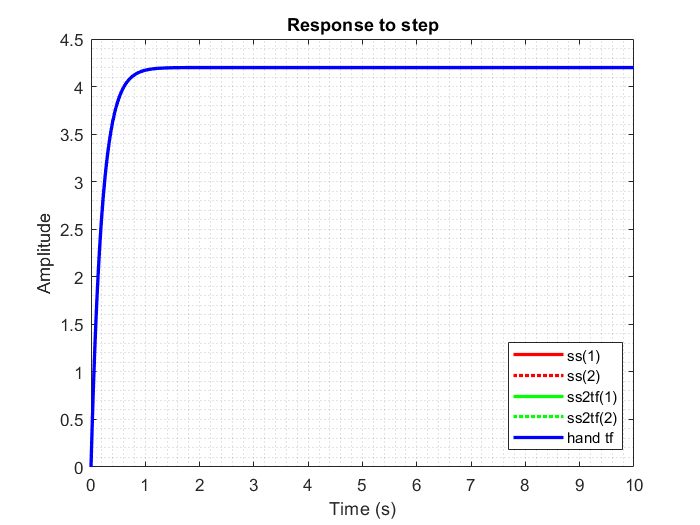
\includegraphics[width=12cm]{images/Q6_b_fig.png}
    \caption{Step Response}
    \label{fig:Q6b}
\end{figure}
\pagebreak